\documentclass[11pt]{article}
\usepackage[utf8]{inputenc} % Para caracteres en espa�ol
\usepackage{amsmath,amsthm,amsfonts,amssymb,amscd}
\usepackage{multirow,booktabs}
\usepackage[table]{xcolor}
\usepackage{fullpage}
\usepackage{lastpage}
\usepackage{enumitem}
\usepackage{multicol}
\usepackage{fancyhdr}
\usepackage{mathrsfs}
\usepackage{wrapfig}
\usepackage{setspace}
\usepackage{esvect}
\usepackage{calc}
\usepackage{multicol}
\usepackage{booktabs}% http://ctan.org/pkg/booktabs
\newcommand{\tabitem}{~~\llap{\textbullet}~~}
\usepackage{cancel}
\usepackage{graphicx}
\graphicspath{ {pictures/} }
\usepackage[retainorgcmds]{IEEEtrantools}
\usepackage[margin=3cm]{geometry}
\usepackage{amsmath}
\newlength{\tabcont}
\setlength{\parindent}{0.0in}
\setlength{\parskip}{0.05in}
\usepackage{empheq}
\usepackage{framed}
\usepackage[most]{tcolorbox}
\usepackage{xcolor}
\colorlet{shadecolor}{orange!15}
\parindent 0in
\parskip 12pt
\geometry{margin=1in, headsep=0.5in}
\theoremstyle{definition}
\newtheorem{defn}{Definition}
\newtheorem{reg}{Rule}
\newtheorem{exer}{Exercise}
\usepackage{setspace}
%\singlespacing
%\onehalfspacing
%\doublespacing
\setstretch{1.5}
\newtheorem{note}{Note}
\begin{document}
\setcounter{section}{0}
 \pagestyle{fancy}
\fancyhf{}
\rhead{AE370: Application Problems}
{\LARGE \bf Application Problem 1a:}\\ \\
\textbf{Compute $\int_{0}^{3}x^2\, \mathrm{d}x$ using the \underline{Rectangle Rule with 1, 2, and 3 subintervals} Compare your result with the exact solution. Compute the relative error, comment on your solution.} \newline
\noindent\rule{16.5cm}{0.4pt}
\newline
%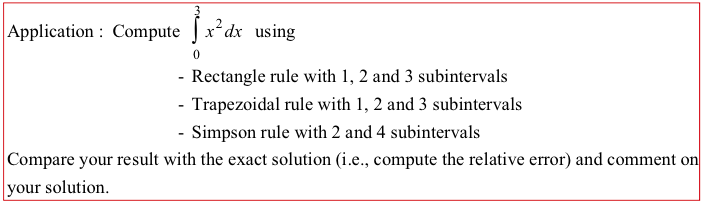
\includegraphics[scale=0.75]{1.png}
\textbf{Exact Solution}
\begin{equation*}
\begin{aligned}
y = \int_{0}^{3} x^2 \mathrm{d}x = \bigg[ \frac{1}{3} x^{3}\bigg]_{0}^{3} = 9
\end{aligned}
\end{equation*}
\newline
\begin{shaded}
\textbf{Rectangle Rule for Integration} \newline
\begin{equation*}
\int_{x_{i-1}}^{x_i} f(x) \mathrm{d}x \approx \sum_{i=1}^{n} \, h \, f(\frac{x_{i-1}+x_{i}}{2})
\end{equation*}
Where:
\begin{equation*}
\begin{split}
n &= \text{Number of Subintervals} \\ \\
h &= \frac{x_{\text{final}} - x_{\text{initial}}}{n} \qquad \text{Length of a Single Subinterval} \\
\end{split}
\end{equation*}
\end{shaded}
\begin{equation*}
\begin{aligned}
\text{1 Subinterval : } &&&\\
& h = \frac{3-0}{1} = 3  &\text{therefore}& \qquad y = 3 \bigg(\frac{0+3}{2}\bigg)^2 = 6.75 \\
\text{2 Subintervals :} & \\
& h = \frac{3-0}{2} = 1.5 &\text{therefore}& \qquad y = 1.5 \bigg(\frac{0+1.5}{2}\bigg)^2 + 1.5 \bigg(\frac{1.5+3}{2}\bigg)^2 = 8.4375 \\
\text{3 Subintervals :} &\\
& h = \frac{3-0}{3} = 1 &\text{therefore}& \qquad  y = 1 \bigg(\frac{0+1}{2}\bigg)^2 + 1\bigg(\frac{1+2}{2}\bigg)^2 + 1\bigg(\frac{2+3}{2}\bigg)^2= 8.75 \\
\end{aligned}
\end{equation*}
\newpage
{\LARGE \bf Application Problem 1b:}\\ \\
\textbf{Compute $\int_{0}^{3}x^2\, \mathrm{d}x$ using the \underline{Trapezoidal Rule with 1, 2, and 3 subintervals} Compare your result with the exact solution. Compute the relative error, comment on your solution.} \newline
\noindent\rule{16.5cm}{0.4pt}
\newline
%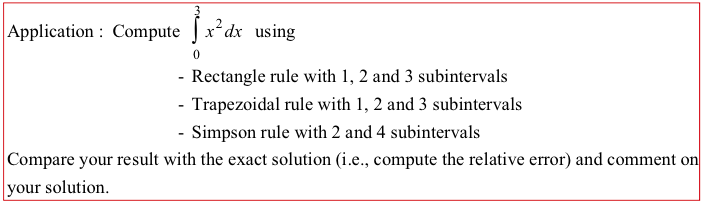
\includegraphics[scale=0.75]{1.png}
\textbf{Exact Solution}
\begin{equation*}
\begin{aligned}
y = \int_{0}^{3} x^2 \mathrm{d}x = \bigg[ \frac{1}{3} x^{3}\bigg]_{0}^{3} = 9
\end{aligned}
\end{equation*}
\\
\begin{shaded}
\textbf{Trapezoidal Rule for Integration} \newline
\begin{equation*}
\int_{x_{i-1}}^{x_i} f(x) \mathrm{d}x \approx \sum_{i=1}^{n} \, \frac{h}{2} \, \bigg(f(x_{i-1})+f(x_{i})\bigg)
\end{equation*}
Where:
\begin{equation*}
\begin{split}
n &= \text{Number of Intervals} \\ \\
h &= \frac{x_{\text{final}} - x_{\text{initial}}}{n} \qquad \text{Length of a Single Subinterval}
\end{split}
\end{equation*}
\end{shaded}
\begin{equation*}
\begin{aligned}
\text{1 Subinterval:} &&&\\
& h = \frac{3-0}{1} = 3  &\text{therefore}& \qquad y = \frac{3}{2}\big(0^2+3^2\big) = 13.5 \\
\text{2 Subintervals:} & \\
& h = \frac{3-0}{2} = 1.5 &\text{therefore}& \qquad y = \frac{1.5}{2}\big(0^2+1.5^2\big)+\frac{1.5}{2}\big(1.5^2+3^2\big) = 10.125 \\
\text{3 Subintervals:} &\\
& h = \frac{3-0}{3} = 1 &\text{therefore}& \qquad  y = \frac{1}{2}\big(0^2+1^2\big)+\frac{1}{2}\big(1^2+2^2\big)+\frac{1}{2}\big(2^2+3^2\big) = 9.5 \\
\end{aligned}
\end{equation*}
\newpage
{\LARGE \bf Application Problem 1c:}\\ \\
\textbf{Compute $\int_{0}^{3}x^2\, \mathrm{d}x$ using the \underline{Simpson Rule with 2 and 4 subintervals} Compare your result with the exact solution. Compute the relative error, comment on your solution.} \newline
\noindent\rule{16.5cm}{0.4pt}
\newline
\textbf{Exact Solution}
\begin{equation*}
\begin{aligned}
y = \int_{0}^{3} x^2 \mathrm{d}x = \bigg[ \frac{1}{3} x^{3}\bigg]_{0}^{3} = 9
\end{aligned}
\end{equation*}
\vspace{0mm}
\begin{shaded}
\textbf{Simpson Rule for Integration} \newline
\begin{equation*}
\int_{x_{i-1}}^{x_i} f(x) \mathrm{d}x \approx \frac{2}{3} \, I_{\text{rectangular}} + \frac{1}{3} \, I_{\text{trapezoidal}}
\end{equation*}
Where:
\begin{equation*}
\begin{split}
I_{\text{rectangular}} &= \text{Rectangle Rule Estimate} \\
I_{\text{trapezoidal}} &= \text{Trapezoidal Rule Estimate} \\
\end{split}
\end{equation*}
\end{shaded}
\vspace{-10mm}
\begin{equation*}
\begin{aligned}
\text{2 Subintervals:} & \\
& h = \frac{3-0}{2} = 1.5 \qquad \text{therefore...} \\ \\
& \qquad I_{\text{rectangular}} = 1.5 \bigg(\frac{0+1.5}{2}\bigg)^2 + 1.5 \bigg(\frac{1.5+3}{2}\bigg)^2 = 8.4375 \\ \\
& \qquad I_{\text{trapezoidal}} = \frac{3-0}{2} = 1.5 = \frac{1.5}{2}\big(0^2+1.5^2\big)+\frac{1.5}{2}\big(1.5^2+3^2\big) = 10.125 \\
\text{As a result}& \\
&\qquad y = \frac{2}{3} \, I_{\text{rectangular}} + \frac{1}{3} \, I_{\text{trapezoidal}} = \frac{2}{3} \, (8.4375) + \frac{1}{3} \, (10.125) = 9
\end{aligned}
\end{equation*}
\newline
This is our exact solution!
\newpage
%%%%%%%%%%%%%%%%%%%%%%%%%%%%%%%%%%%%%%%%%%%%%%%%%%%%%%%%
%%%%%%%%%%%%%%%%%         APPLICATION PROBLEM 2       %%%%%%%%%%%%%%%%%%%%
%%%%%%%%%%%%%%%%%%%%%%%%%%%%%%%%%%%%%%%%%%%%%%%%%%%%%%%%
{\LARGE \bf Application Problem 2a:}\\ \\
\textbf{Compute $\int_{0}^{3} x^2 \mathrm{d}x$ using the 1-point, 2-point Gauss Quadrature Rule. Compare your result with the exact solution (ie. compute the relative error) and comment on your solution} \newline
\noindent\rule{16.5cm}{0.4pt}
\begin{itemize}
\item \textbf{Exact Solution}
\\
\begin{equation*}
\begin{aligned}
y = \int_{0}^{3} x^2 \mathrm{d}x = \bigg[ \frac{1}{3} x^{3}\bigg]_{0}^{3}
\end{aligned}
\end{equation*}
\item \textbf{1 Point Gauss Quadrature Rule} 
\\ \\ 
Such that $w_1 = 2$ and $\xi_1 = 0$: 
\\
\begin{equation*}
\begin{aligned}
I = \int_{0}^{3} x^2 \mathrm{d}x &= \frac{3}{2}\int_{-1}^1 f\bigg(\frac{3\xi + 3}{2}\bigg)\mathrm{d}\xi \\ \\
& = \frac{3}{2}\int_{-1}^1 \bigg(\frac{3\xi + 3}{2}\bigg)^2\mathrm{d}\xi \\ \\
& = 2 \bigg(\frac{3 \,(0) + 3}{2}\bigg)^2 = \frac{18}{4} = 4.5
\end{aligned}
\end{equation*}
\item \textbf{2 Point Gauss Quadrature Rule}
\begin{equation*}
\begin{aligned}
\text{Such that } w_1 = w_2 = 1 \text{ , } &\xi_1 = -\frac{\sqrt{3}}{3} \text{ and } \xi_2 = \frac{\sqrt{3}}{3} \text{ :}\qquad \qquad \qquad \qquad \qquad \qquad \qquad \qquad \qquad \qquad \qquad \qquad \qquad \qquad \qquad
\end{aligned}
\end{equation*}
\begin{equation*}
\begin{aligned}
I &= w_1 \, f(\xi_1) + w_2 \, f(\xi_2) \\ \\
& = \frac{3}{2}\bigg(\frac{3 \,(-\frac{\sqrt{3}}{3}) + 3}{2}\bigg)^2 + \, \frac{3}{2}\bigg(\frac{3 \,(\frac{\sqrt{3}}{3}) + 3}{2}\bigg)^2 \\ \\
& = 9
\end{aligned}
\end{equation*}
\end{itemize}
\newpage
%%%%%%%%%%%%%%%%%%%%%%%%%%%%%%%%%%%%%%%%%%%%%%%%%%%%%%%%
%%%%%%%%%%%%%%%%%         APPLICATION PROBLEM 2       %%%%%%%%%%%%%%%%%%%%
%%%%%%%%%%%%%%%%%%%%%%%%%%%%%%%%%%%%%%%%%%%%%%%%%%%%%%%%
{\LARGE \bf Application Problem 2b:}\\ \\
\textbf{Compute $\int_{-\frac{\pi}{2}}^{\frac{\pi}{2}} \cos(x) \mathrm{d}x$ using the 1-point, 2-point Gauss Quadrature Rule. Compare your result with the exact solution (ie. compute the relative error) and comment on your solution}\newline
\noindent\rule{16.5cm}{0.4pt}
\begin{itemize}
\item \textbf{Exact Solution}
\\
\begin{equation*}
\begin{aligned}
y = \int_{-\frac{\pi}{2}}^{\frac{\pi}{2}} \cos(x) \mathrm{d}x = \bigg[ \sin(x)\bigg]_{-\frac{\pi}{2}}^{\frac{\pi}{2}} = 2
\end{aligned}
\end{equation*}
\\
First we must do a Coordinate Transformation to get this in the form we want.
\\
\begin{equation*}
\begin{aligned}
\int_{-\frac{\pi}{2}}^{\frac{\pi}{2}} \cos(x) \mathrm{d}x = \frac{\pi}{2} \int_{-1}^{1} \cos \bigg(\frac{\pi}{2} \, \xi \bigg) \mathrm{d}\xi
\end{aligned}
\end{equation*}
\\
\item \textbf{1 Point Gauss Quadrature Rule} 
Such that $w_1 = 2$ and $\xi_1 = 0$:
\begin{equation*}
\begin{aligned}
I &= \frac{\pi}{2} \bigg[ \cos (\frac{\pi}{2} \, \xi_1) \, w_1\bigg] \\ \\
& = \frac{\pi}{2} \bigg[ \cos \big(\frac{\pi}{2} \, (0)\big) \, 2\bigg] \\ \\
& = 3.14
\end{aligned}
\end{equation*}
\newpage
\item \textbf{2 Point Gauss Quadrature Rule}
\begin{equation*}
\begin{aligned}
\text{Such that } w_1 = w_2 = 1 \text{ , } &\xi_1 = -\frac{\sqrt{3}}{3} \text{ and } \xi_2 = \frac{\sqrt{3}}{3} \text{ :} \qquad \qquad \qquad \qquad \qquad \qquad \qquad \qquad \qquad \qquad \qquad \qquad \qquad \qquad \qquad
\end{aligned}
\end{equation*}
\\
\begin{equation*}
\begin{aligned}
I &= \frac{\pi}{2} \bigg[ w_1 \, \cos (\frac{\pi}{2} \, \xi_1) + w_2 \, \cos (\frac{\pi}{2} \, \xi_2) \bigg] \\ \\
& = \frac{\pi}{2} \Bigg[1 \, \cos \Big(\frac{\pi}{2} \, (-\frac{\sqrt{3}}{3})\Big) \, + 1 \, \cos \Big(\frac{\pi}{2} \, (\frac{\sqrt{3}}{3})\Big)\Bigg] \\ \\
& = 1.9352 \quad \approx 3 \% \text{ off}
\end{aligned}
\end{equation*}
\\ \\
The solution alternates between over estimate and under estimate.
\end{itemize}
\newpage
%%%%%%%%%%%%%%%%%%%%%%%%%%%%%%%%%%%%%%%%%%%%%%%%%%%%%%%%
%%%%%%%%%%%%%%%%%         APPLICATION PROBLEM 3       %%%%%%%%%%%%%%%%%%%%
%%%%%%%%%%%%%%%%%%%%%%%%%%%%%%%%%%%%%%%%%%%%%%%%%%%%%%%%
{\LARGE \bf Application Problem 3:}\\ \\
\textbf{Compute $\int_{-1}^{1}\int_{-1}^{1} \exp(2x)*\ln(3+y)\mathrm{d}y\mathrm{d}x$ using the $1*1$, $2*2$, $3*3$ Gauss Quadrature rule. Compare your result with the exact solution $(I_{ex} = 7.829967)$. Compute the relative error and comment on your solution.} \newline
\noindent\rule{16.5cm}{0.4pt}
\begin{itemize}
\item \textbf{Exact Solution}
\begin{equation*}
\begin{aligned}
I_{\text{exact}} = \int_{-1}^{1} \int_{-1}^{1} e^{2 \, x} \cdot \ln(3+y) \, \mathrm{d}y \, \mathrm{d}x = 7.829967
\end{aligned}
\end{equation*}
\item \textbf{1*1 Point Gauss Quadrature Rule} 
Such that $w = w_1 \times w_1 = 4$ and $\xi_1 = \eta_1 = 0$:
\begin{equation*}
\begin{aligned}
I &= w \, f(\xi_1, \eta_1) \\ \\
& = 4 \, e^{0} \cdot \ln (3) = 4.39449
\end{aligned}
\end{equation*}
\item \textbf{2*2 Point Gauss Quadrature Rule}
\begin{equation*}
\begin{aligned}
\text{Such that } w_k = 1 \text{ and } & (\xi_k, \eta_k) = \big(\pm \frac{\sqrt{3}}{3}, \pm \frac{\sqrt{3}}{3} \big)\text{ :} \qquad \qquad \qquad \qquad \qquad \qquad \qquad \qquad \qquad \qquad \qquad \qquad \qquad \qquad \qquad
\end{aligned}
\end{equation*}
\begin{equation*}
\begin{aligned}
I &= \sum w_k \, f(\xi_k, \eta_k) \\ \\
& = 1 \, \exp \Bigg[2 \, \Big(-\frac{\sqrt{3}}{3}\Big)\Bigg] \, \ln \Bigg(3 +\, \Big(-\frac{\sqrt{3}}{3}\Big)\Bigg) 
& +\quad 1 \, \exp \Bigg[2 \, \Big(-\frac{\sqrt{3}}{3}\Big)\Bigg] \, \ln \Bigg(3 +\Big(\frac{\sqrt{3}}{3}\Big)\Bigg)\\ \\
& \qquad \quad + 1 \, \exp \Bigg[2 \, \Big(\frac{\sqrt{3}}{3}\Big)\Bigg] \, \ln \Bigg(3 +\Big(\frac{\sqrt{3}}{3}\Big)\Bigg) 
& +\quad 1 \, \exp \Bigg[2 \, \Big(\frac{\sqrt{3}}{3}\Big)\Bigg] \, \ln \Bigg(3 +\Big(-\frac{\sqrt{3}}{3}\Big)\Bigg)\\ \\
& = 7.532767
\end{aligned}
\end{equation*}
\end{itemize}
\newpage
{\LARGE \bf Application Problem 4:}\\ \\
Derive the second-order central difference approximations of the first and second derivatives
\newpage
{\LARGE \bf Application Problem 5:}\\ \\
Let $f(x) = \sin (x)$. Compute $f'(1)$ using the \underline{Forward Difference Scheme} with $h = 0.25$ and $h = 0.5$. Then Improve your solution by using the \underline{Richardson's Extrapolation Scheme}. Compare your three approximations with the exact solution.
\begin{shaded}
\textbf{Forward Difference Scheme}
\begin{equation*}
\begin{aligned}
f'(x) = \frac{f(x+h)-f(x)}{h} - \frac{h}{2} f''(\xi) \qquad \text{with } \xi \in (x,x+h)
\end{aligned}
\end{equation*}
\end{shaded}
\begin{itemize}
\item Exact
\begin{equation*}
\begin{aligned}
f'(1)_{\text{exact}} = 0.5403 
\end{aligned}
\end{equation*}
\item h=0.25
\begin{equation*}
\begin{aligned}
f'(x) = \frac{\sin(x+0.25) - \sin(x)}{0.25} \quad \rightarrow \quad f'(x) = 0.43055
\end{aligned}
\end{equation*}
\item h=0.50
\begin{equation*}
\begin{aligned}
f'(x) = \frac{\sin(x+0.5) - \sin(x)}{0.5} \quad \rightarrow \quad f'(x) = 0.312048
\end{aligned}
\end{equation*}
\end{itemize}
\begin{shaded}
\textbf{Richardson Extrapolation}
\begin{equation*}
\begin{aligned}
a_o = F(h) + \frac{F(h) - F(qh)}{q^p - 1} + O(h^r) \qquad \text{or} \qquad a_o = \frac{F(qh) - q^p\,F(h)}{1 - q^p}+ O(h^2)
\end{aligned}
\end{equation*}
\end{shaded}
For this problem
\begin{equation*}
\begin{aligned}
h &= 0.25 \quad &f'(1) = 0.430551 = F(h)\\
h &= 0.50 \quad &f'(1) = 0.312048 = F(qh)
\end{aligned}
\end{equation*}
Where $q=2$ and $p=1$ since we are using the Forward Difference Scheme and error (h) is linear.
\begin{equation*}
\begin{aligned}
a_o = \frac{F(qh) - q\,F(h)}{1 - q} = \frac{0.312048 - 2 \,(0.430551)}{1-2} = 0.54806
\end{aligned}
\end{equation*}
\newpage
{\LARGE \bf Application Problem 6:}\\ \\
Let $f(x) = \exp(1+3 \, x)$. Compute $f'(2)$ using the \underline{Central Difference Scheme} with $h = 0.04$ and $h = 0.08$. Then Improve your solution by using the \underline{Richardson's Extrapolation scheme}. Compare your three approximations with the exact solution.
\begin{shaded}
\textbf{Central Difference Scheme}
\begin{equation*}
\begin{aligned}
f'(x) = \frac{f(x+h)-f(x-h)}{2h} - \frac{h^2}{6} f'''(\xi) \qquad \text{with } \xi \in (x,x+h)
\end{aligned}
\end{equation*}
\end{shaded}
\vspace{-10mm}
\begin{itemize}
\item Exact
\begin{equation*}
\begin{aligned}
f'(2)_{\text{exact}} = 3289.899 
\end{aligned}
\end{equation*}
\item h=0.04
\begin{equation*}
\begin{aligned}
f'(2) = F(h) = \frac{\exp(1+3\,(2+0.04))-\exp(1+3\,(2-0.04))}{2\,(0.04)} = 3297.801
\end{aligned}
\end{equation*}
\item h=0.08
\begin{equation*}
\begin{aligned}
f'(2) = F(qh) = \frac{\exp(1+3\,(2+0.08))-\exp(1+3\,(2-0.08))}{2\,(0.08)} = 3321.574
\end{aligned}
\end{equation*}
\end{itemize}
\begin{shaded}
\textbf{Richardson Extrapolation}
\begin{equation*}
\begin{aligned}
a_o = F(h) + \frac{F(h) - F(qh)}{q^p - 1} + O(h^r) \qquad \text{or} \qquad a_o = \frac{F(qh) - q^p\,F(h)}{1 - q^p}+ O(h^2)
\end{aligned}
\end{equation*}
\end{shaded}
For this problem
\begin{equation*}
\begin{aligned}
h &= 0.04 \quad &f'(2) = 3297.801 = F(h)\\
h &= 0.08 \quad &f'(2) = 3321.574 = F(qh)
\end{aligned}
\end{equation*}
Where $q=2$ and $p=2$ since we are using the Central Difference Scheme and error (h) is squared
\begin{equation*}
\begin{aligned}
a_o = \frac{F(qh) - q^2\,F(h)}{1 - q^2} = \frac{3321.574 - 4 \,(3297.801)}{1-4} = 3289.877
\end{aligned}
\end{equation*}
\newpage
%%%%%%%%%%%%%%%%%%%%%%%%%%%%%%%%%%%%%%%%%%%%%%%%%%%%%%%%
%%%%%%%%%%%%%%%%%         APPLICATION PROBLEM 7       %%%%%%%%%%%%%%%%%%%%
%%%%%%%%%%%%%%%%%%%%%%%%%%%%%%%%%%%%%%%%%%%%%%%%%%%%%%%%
{\LARGE \bf Application Problem 7:}\\ \\
\textbf{Transform the mass/spring/dashpot equation}
\begin{equation*}
\begin{aligned}
\bf{m\,x'' = m\,g - k\,x - c\,x'}
\end{aligned}
\end{equation*}
\textbf{into a system of $1^{st}$ -order ODE.} \newline
\noindent\rule{16.5cm}{0.4pt}
\newline
\begin{equation*}
\begin{aligned}
m \frac{\mathrm{d}^2x }{\mathrm{d} t^2} = mg - kx - c\frac{\mathrm{d} x}{\mathrm{d} t}
\end{aligned}
\end{equation*}

Divide by m in order to isolate the second order term.

\begin{equation*}
\begin{aligned}
\frac{\mathrm{d}^2x }{\mathrm{d} t^2} = g - \frac{k}{m}\,x - \frac{c}{m}\frac{\mathrm{d} x}{\mathrm{d} t}
\end{aligned}
\end{equation*}

Lets say $y=\frac{\mathrm{d} x}{\mathrm{d} t}$ Therefore...

\begin{equation*}
\begin{aligned}
\frac{\mathrm{d} y }{\mathrm{d} t} = g - \frac{k}{m}\,x - \frac{c}{m}\,y
\end{aligned}
\end{equation*}

Where

\begin{equation*}
\begin{aligned}
y=\frac{\mathrm{d} x}{\mathrm{d} t}
\end{aligned}
\end{equation*}

We have transformed the second order ODE into two coupled first order ODE.

\newpage
%%%%%%%%%%%%%%%%%%%%%%%%%%%%%%%%%%%%%%%%%%%%%%%%%%%%%%%%
%%%%%%%%%%%%%%%%%         APPLICATION PROBLEM 8       %%%%%%%%%%%%%%%%%%%%
%%%%%%%%%%%%%%%%%%%%%%%%%%%%%%%%%%%%%%%%%%%%%%%%%%%%%%%%
{\LARGE \bf Application Problem 8:}\\ \\
\textbf{Use Euler Scheme to solve}
\begin{equation*}
\begin{aligned}
\bf{y' = y \qquad \textbf{on} \qquad 0\leq t \leq 4} \qquad \textbf{with} \qquad y(0) = 1
\end{aligned}
\end{equation*}
\textbf{Use h=1 and compute the relative error at t=4} \newline
\noindent\rule{16.5cm}{0.4pt}
\end{document}